%\section{Results}
%\label{sec:Results}
%% Results should be clear and concise.

The experiment to test the hypothesis that participants in a virtual reality (VR) experiment would show a trend towards choosing complex environments over simple ones when given the task of identifying the more comfortable facade design, was conducted at the Kyushu University campus in Fukuoka, Japan, over a period of 15 days, from October 12 to 30, 2023, during the work hours between 10:00 and 18:00.

A total of \(10\) participants took part in the experiment, primarily consisting of university students and faculty members.
The participants had diverse professional backgrounds, as shown in Figure \ref{fig:SurveyBackgroundChart}, with over \(67\%\) being students from various faculties, approximately \(33\%\) having a construction background, and \(14\%\) reporting previous experience in facade design, as indicated in Figure \ref{fig:SurveyYearsExperienceChart}

%% Participant background chart and years of experience
    \begin{table*}[htb]
        \centering
        \small
        \begin{tabularx}{\textwidth}{X X}
            \centering
            % trim=left 0 down 50 right 0 top 50
            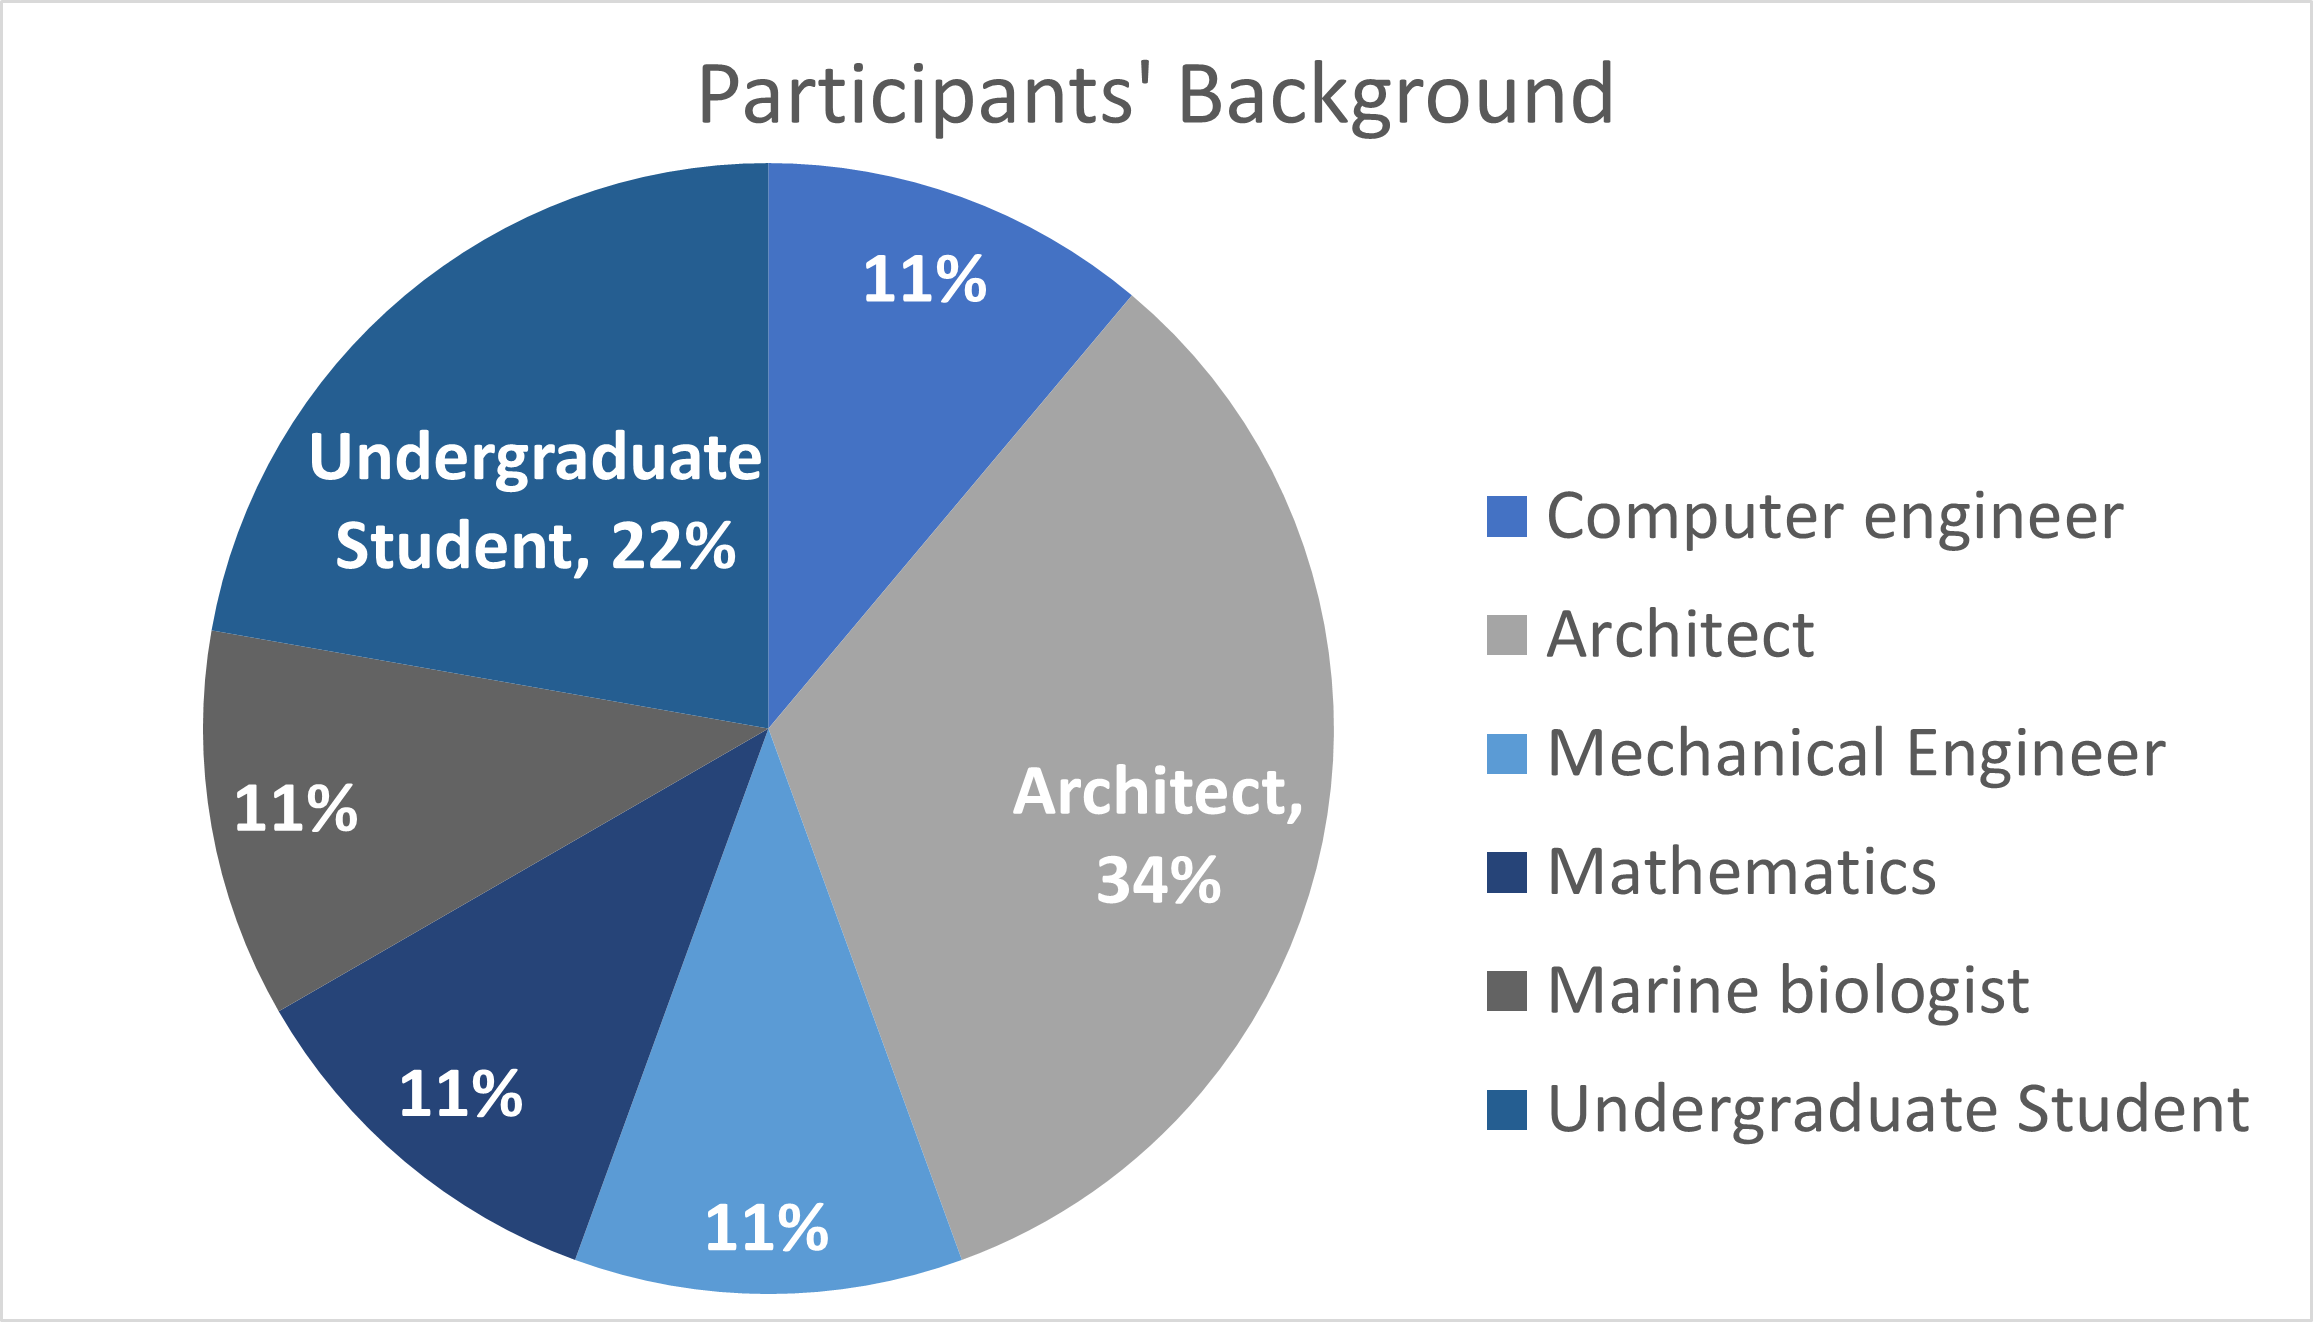
\includegraphics[width=\linewidth, trim=0 60 0 0]{Images/SurveyBackground}
            \captionof{figure}{This chart shows the professional backgrounds of participants involved in the facade design complexity analysis experiment.}
            \label{fig:SurveyBackgroundChart} &
            \centering
            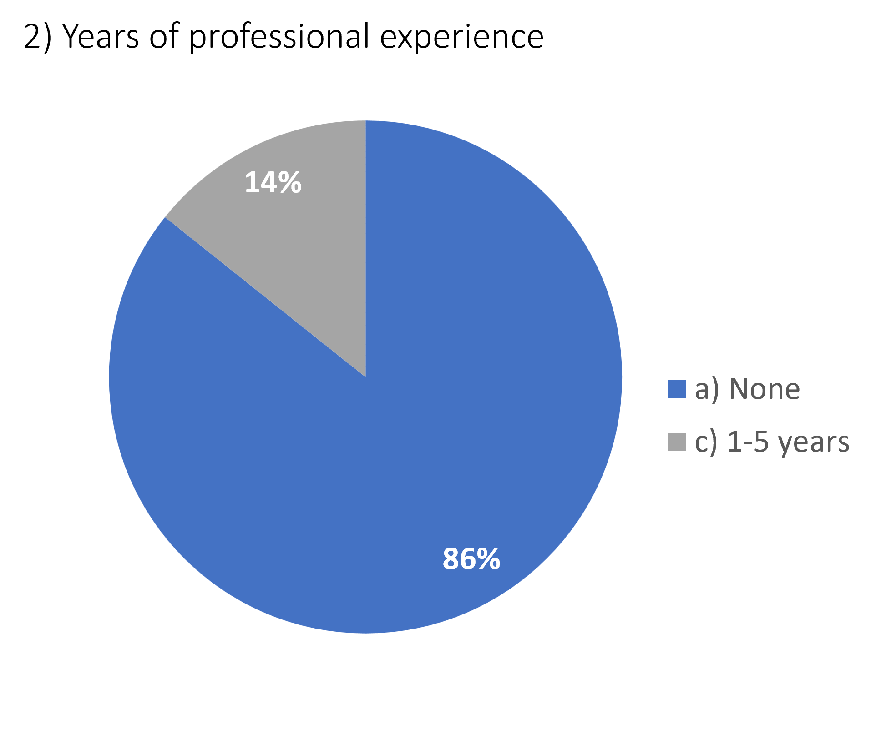
\includegraphics[width=\linewidth, trim=0 60 0 0]{Images/SurveyExperience}
            \captionof{figure}{This chart displays the experience levels in facade design of participants for the study complexity analysis in building design.}
            \label{fig:SurveyYearsExperienceChart}
        \end{tabularx}
    \end{table*}

In the `VR Interaction' stage, which focused on assessing user tolerance for complex facade designs, each participant completed the facade selection task for all three patterns, resulting in a total of 30 experiment sessions.
For each pattern, participants provided one answer, indicating their preference for the facade variation labeled with a complexity level that they found the most comfortable.

%!Complexity level chosen bar chart

The results of participants' preferred complexity levels during the VR simulation stage of the experiment were consolidated into a bar chart titled the ``Complexity Level Chosen Chart,'' shown in Figure \ref{fig:ComplexityLevelChosenChart}.

    % Complexity level chosen Chart
    \begin{figure}[htb]
        \centering
        %trim=100 180 100 120, clip
        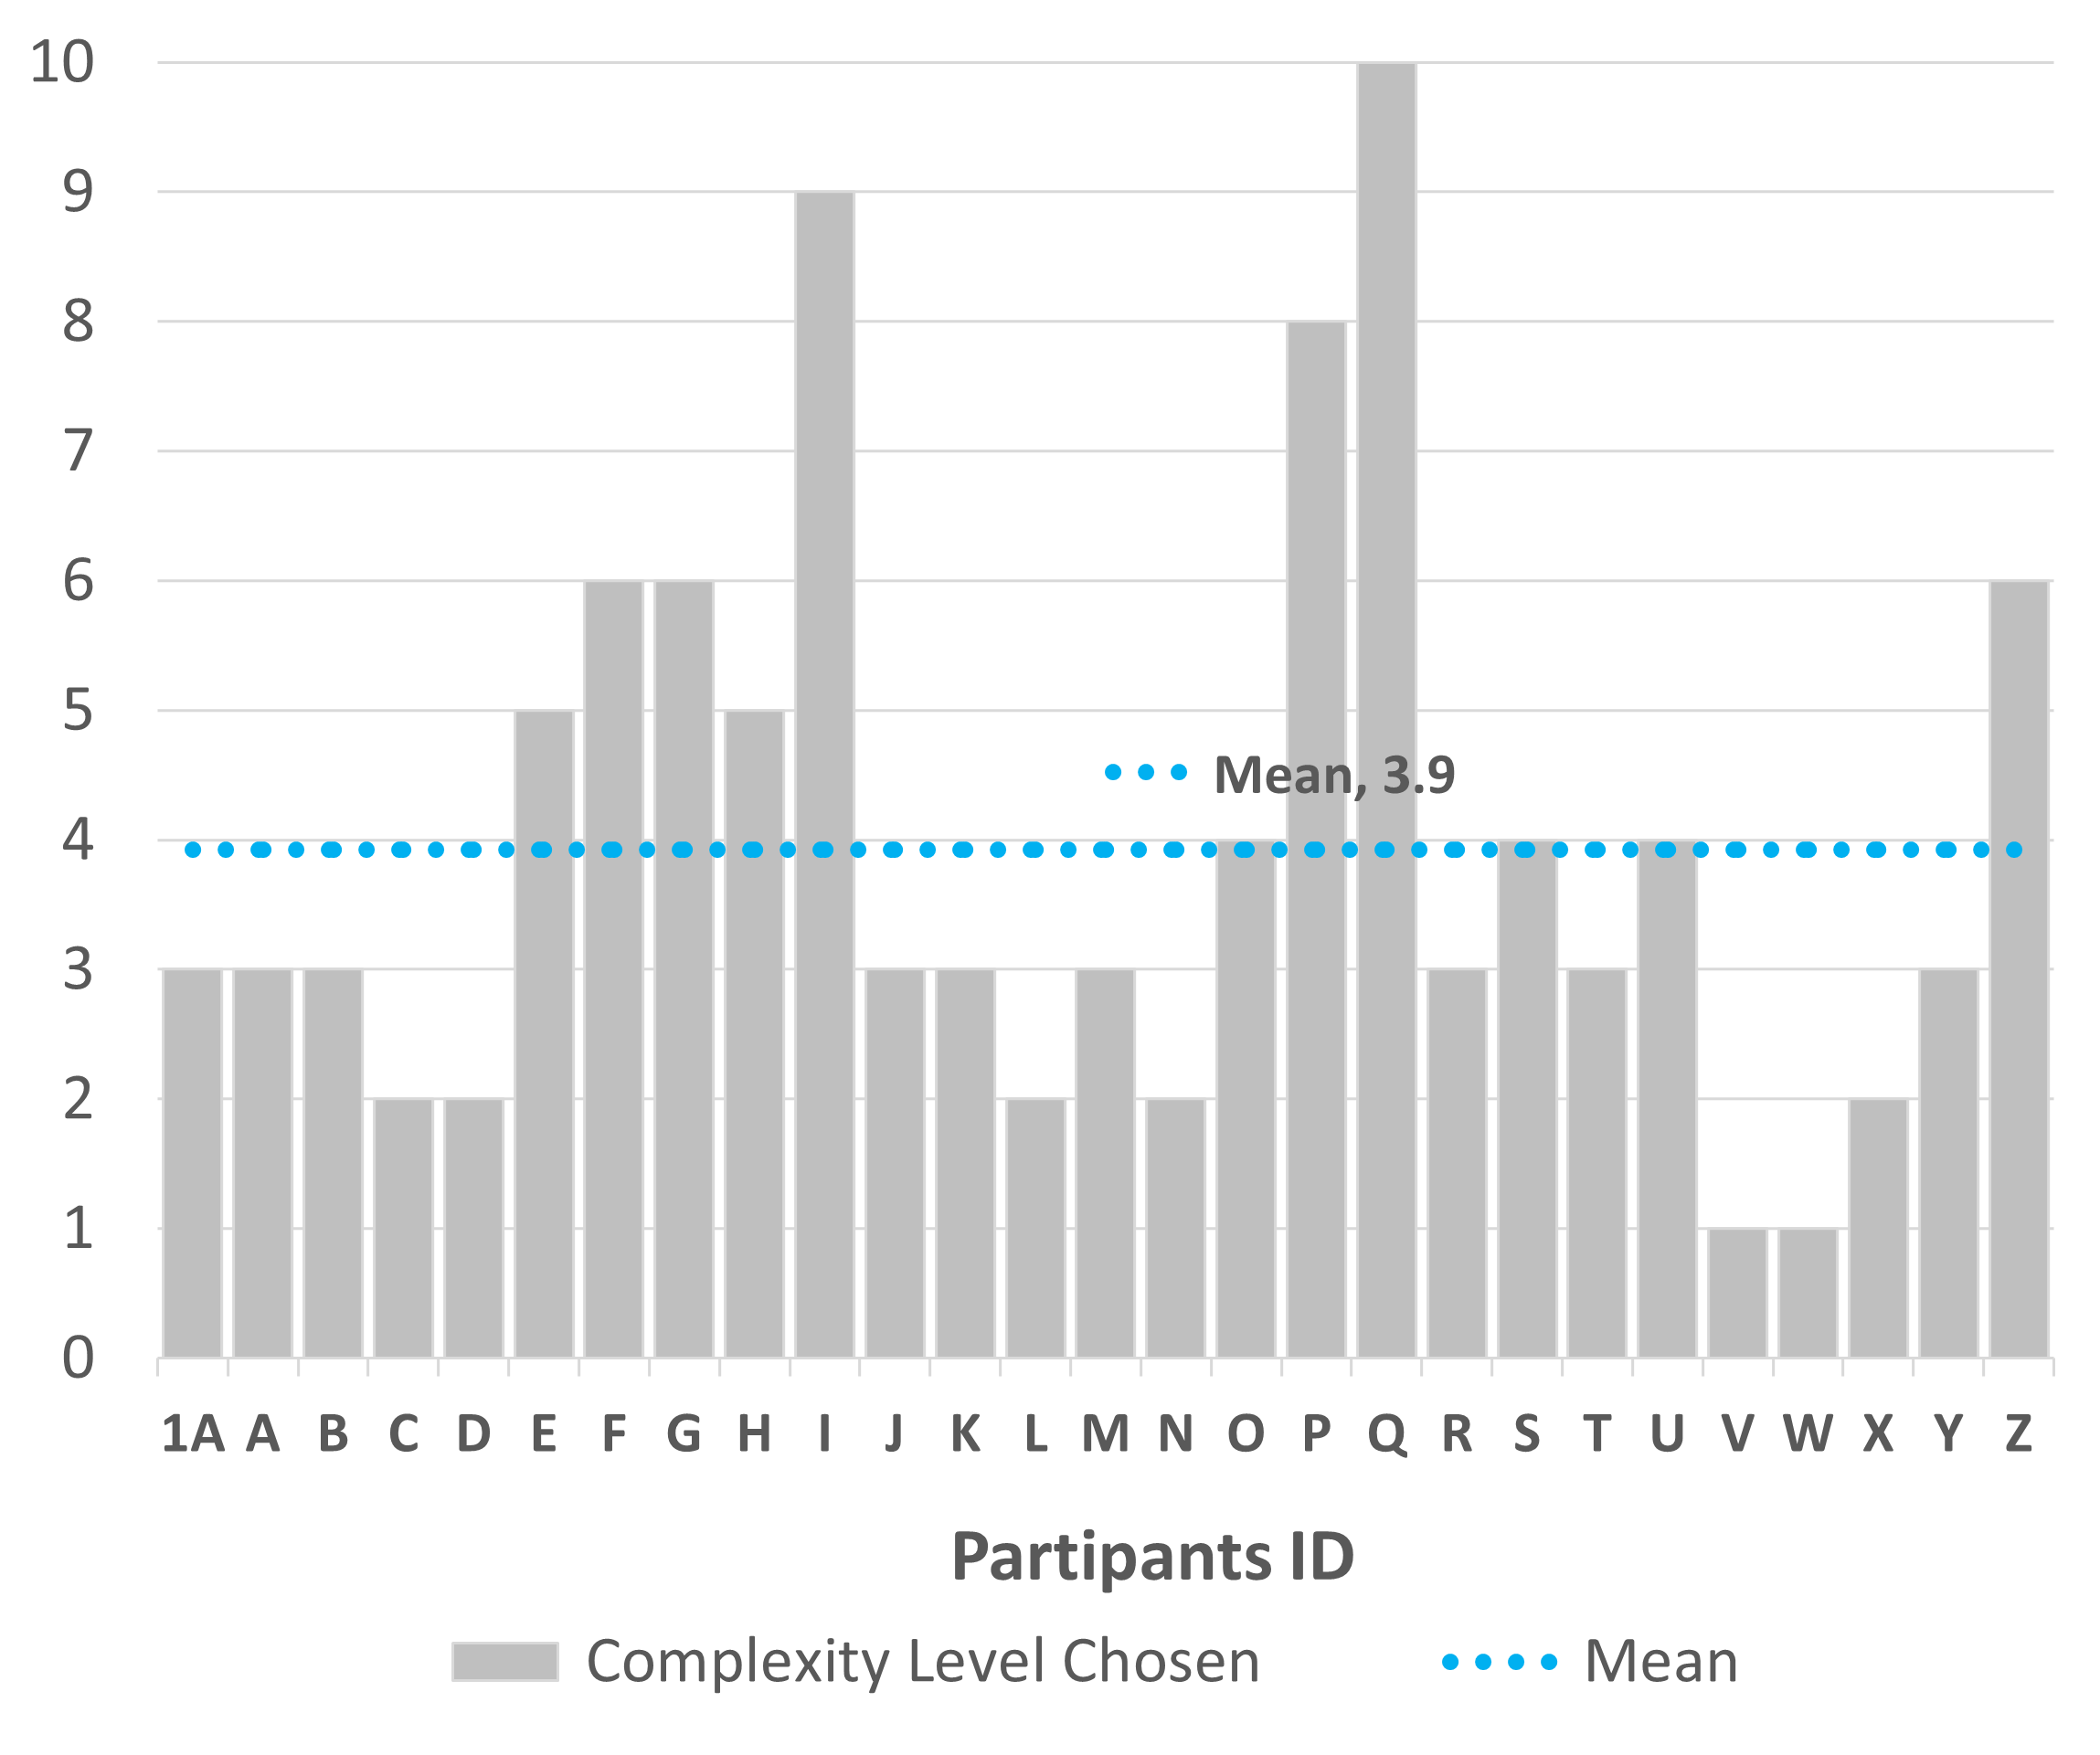
\includegraphics[width=\linewidth]{Images/ComplexityLevelChosenChart}
        \caption{Chart displaying participants' preferred complexity levels among the ten options during the VR simulation stage of the experiment for all three patterns.(Complexity Score: Mean = 3.82; SD = 1.1)}
        \label{fig:ComplexityLevelChosenChart}
    \end{figure}

Analysis of the ``Complexity Level Chosen Chart,'' represented in Figure \ref{fig:ComplexityLevelChosenChart}, reveals a diverse spectrum of preferences across the 30 experiment sessions.
Most participants opted for one of the first five facade variations, with only five instances selecting options beyond this range.
This choice means that on average, participants favored a complexity score level of \(Mean = 3.82\), as determined by the Computational Image Complexity Analysis (CICA) system, with a standard deviation of \(SD = 1.1\).
 Interestingly, ``facade variation 3'' emerged as the most popular choice for all three patterns among the ten defined complexity levels.

%!Complexity level chosen probability graph

The Probability Complexity Level Graph, showcased in Figure \ref{fig:ProbabilityComplexitylevelChart}, provides a visual representation of the distribution of participant choices.
It accentuates that there is a \(40\%\) probability of the focus group selecting an answer proximate to the calculated complexity score average,\(Mean = 3.82\) with a modest standard deviation of \(SD = 13\%\) in predicting individual data points or outcomes.

     % Probability Chart and Complexity level per Pattern
    \begin{table*}[htb]
        \centering
        \small
        \begin{tabularx}{\textwidth}{X X}
            \centering
            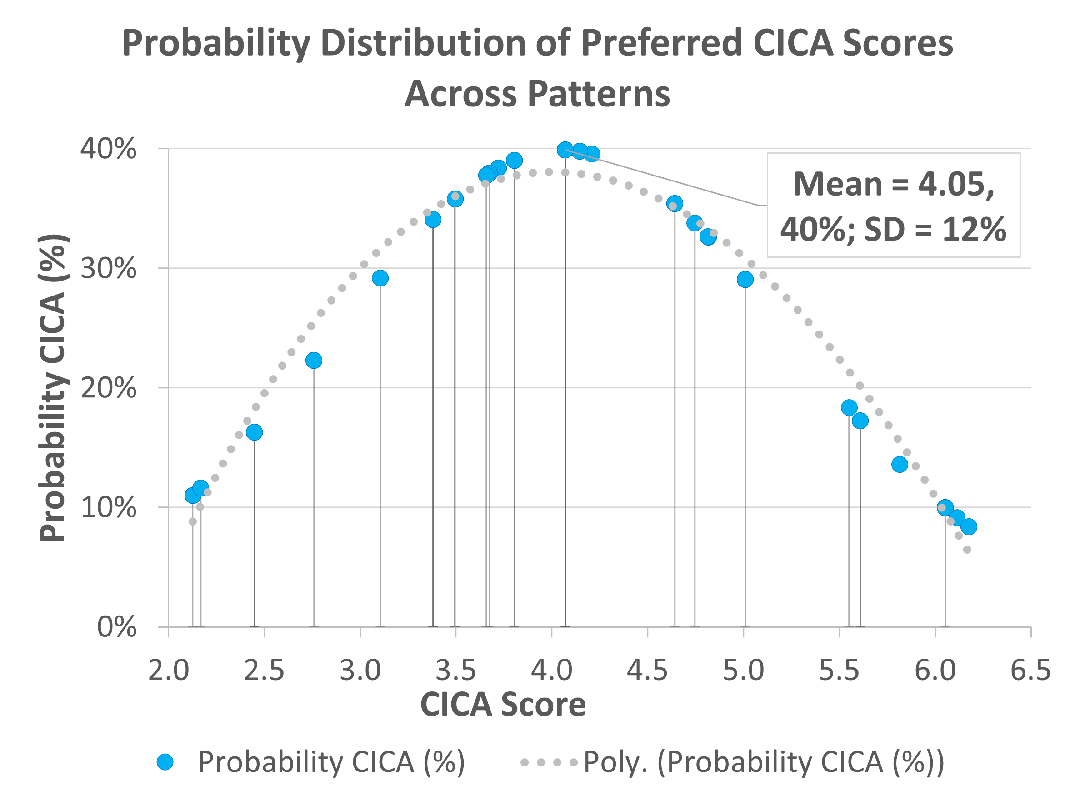
\includegraphics[width=\linewidth, trim=0 0 0 20]{Images/ProbabilityPreferredComplexitylevel}
            \captionof{figure}{Scatter graph illustrating the probability distribution of preferred complexity levels for facade design across all three patterns, derived from data collected during the VR stage of the experiment.(Probability Complexity score: \(Mean = 3.82, 40\%\ ; SD = 13\%\))}
            \label{fig:ProbabilityComplexitylevelChart} &
            \centering
            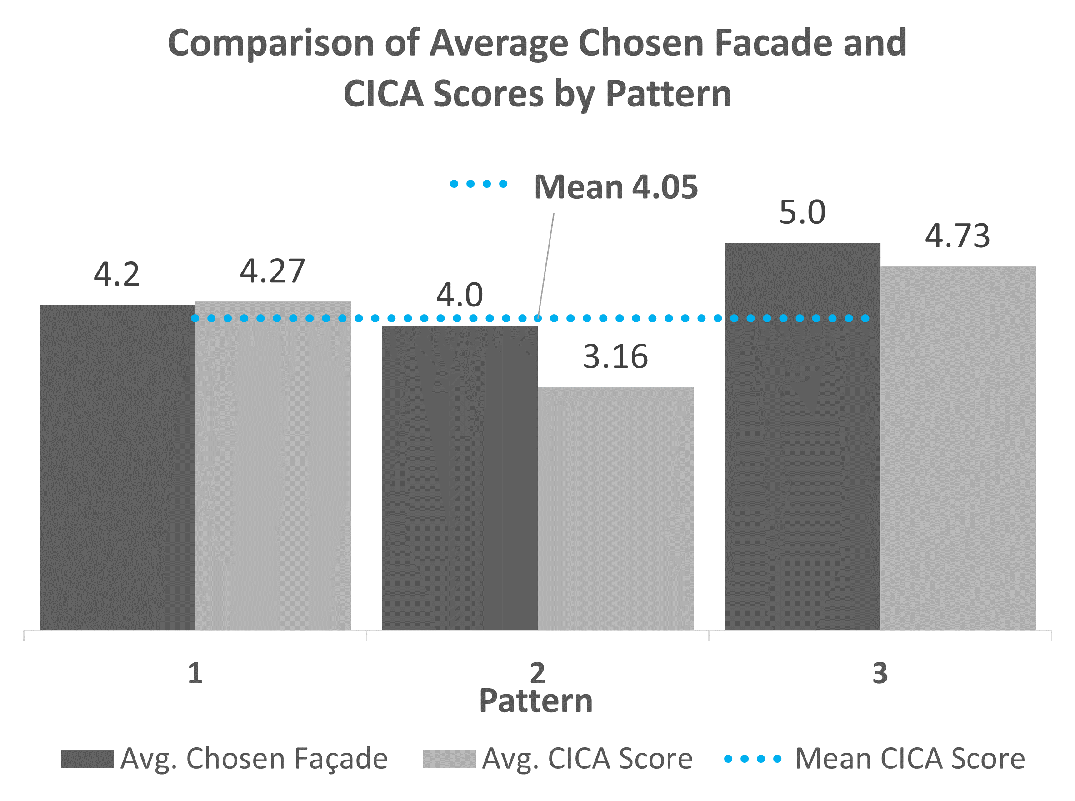
\includegraphics[width=\linewidth, trim=0 0 0 20]{Images/PreferredComplexityLevelPerPattern}
            \captionof{figure}{Average complexity score of preferred facade variation per pattern chosen by participants during the VR simulation (Facade variation: \(Mean = 3.9\). Complexity score: \(Mean = 3.82; SD = 1.1\)).}
            \label{fig:ComplexityLevelPerPattern}
        \end{tabularx}
    \end{table*}


%!Complexity level per pattern graph

The Complexity Level Per Pattern Chart, displayed in Figure \ref{fig:ComplexityLevelPerPattern}, underscores that the average choice of facade variation for each pattern hovers around the overall average complexity score,\(Mean = 3.82\) and the average choice of facade variation \(Mean = 3.9\).
These findings indicate that the most favored facade selections per pattern consistently fall within the range of the overall average complexity score.

%!Complexity perception per level with trendlines

In terms of the accuracy of the 'Computational Image Complexity Analysis' (CICA) system in assessing the complexity of facade variations in comparison to participant perceptions, our findings are visually represented in Figures \ref{fig:AccuracyPattern1}, \ref{fig:AccuracyPattern2}, and \ref{fig:AccuracyPattern3}.
These figures illustrate that the trendlines for all three patterns closely mirror the trajectory of the trendline derived from the original ranking data.
The average standard deviation across these comparisons is \(SD = 1.1\) in complexity level categorization.

  %% Complexity Perception Survey results
    \begin{table*}[htb]
        \centering
        \small
        \begin{tabularx}{\textwidth}{X X X}
            \centering
            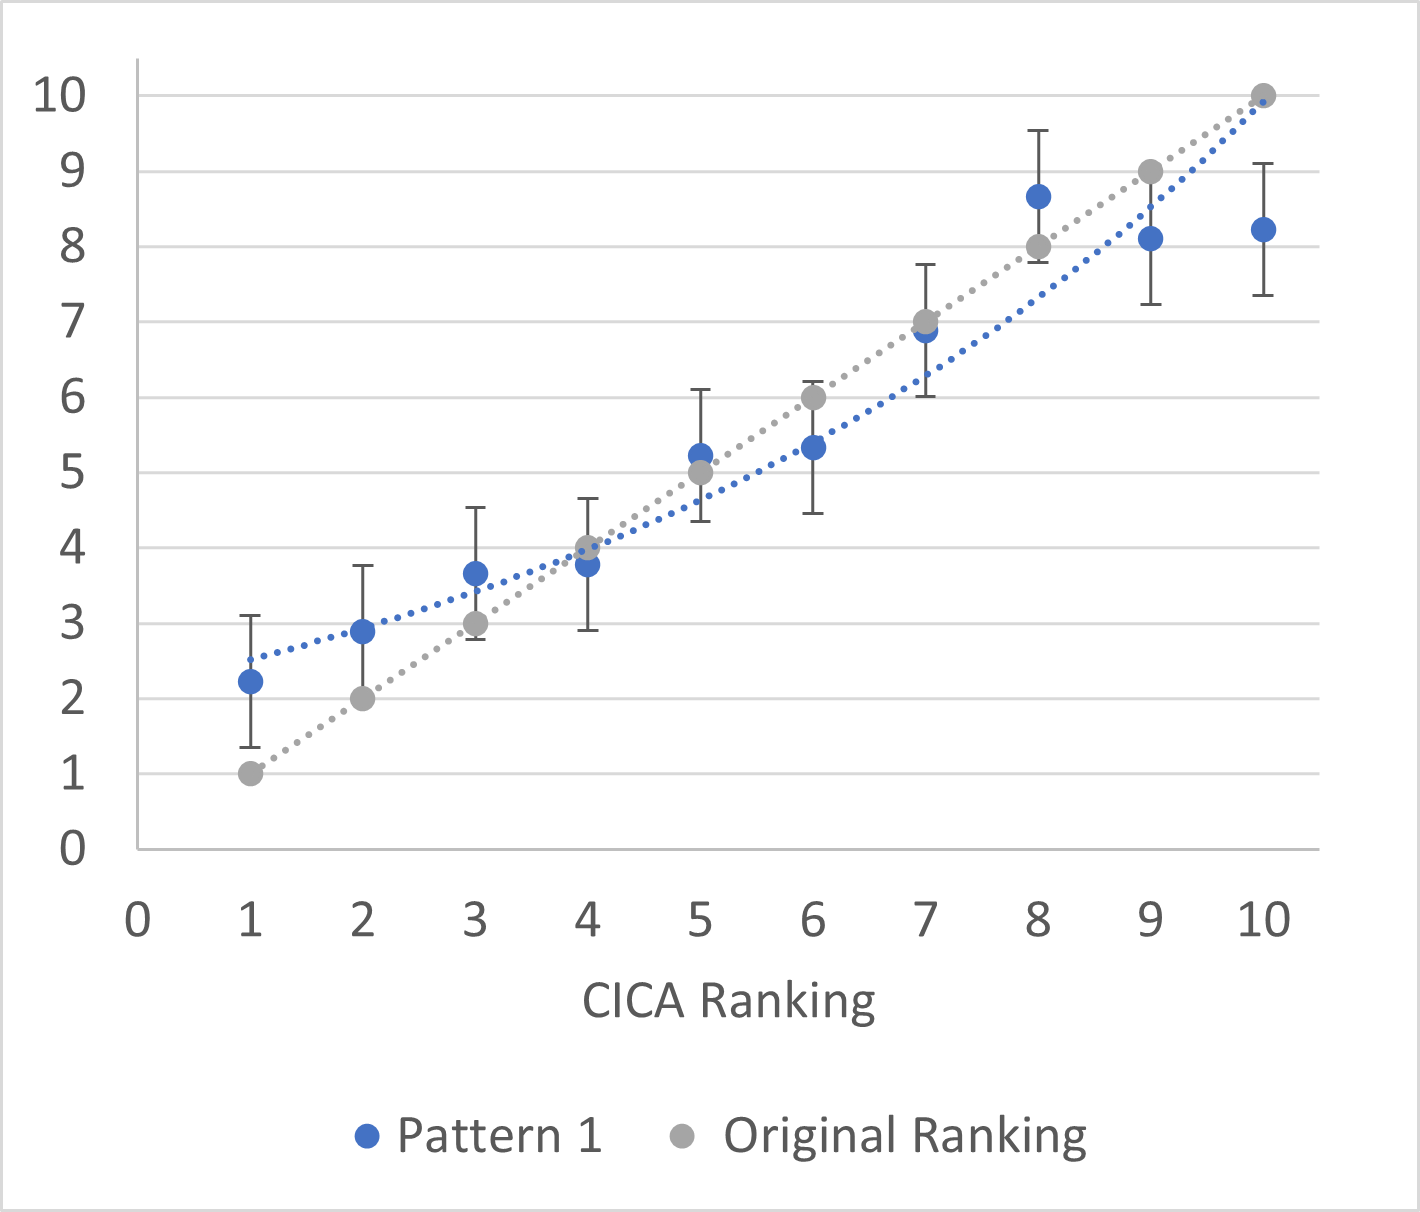
\includegraphics[width=\linewidth]{Images/AccuracyPattern1}
            \captionof{figure}{Accuracy comparison pattern 1 with original ranking}
            \label{fig:AccuracyPattern1} &
            \centering
            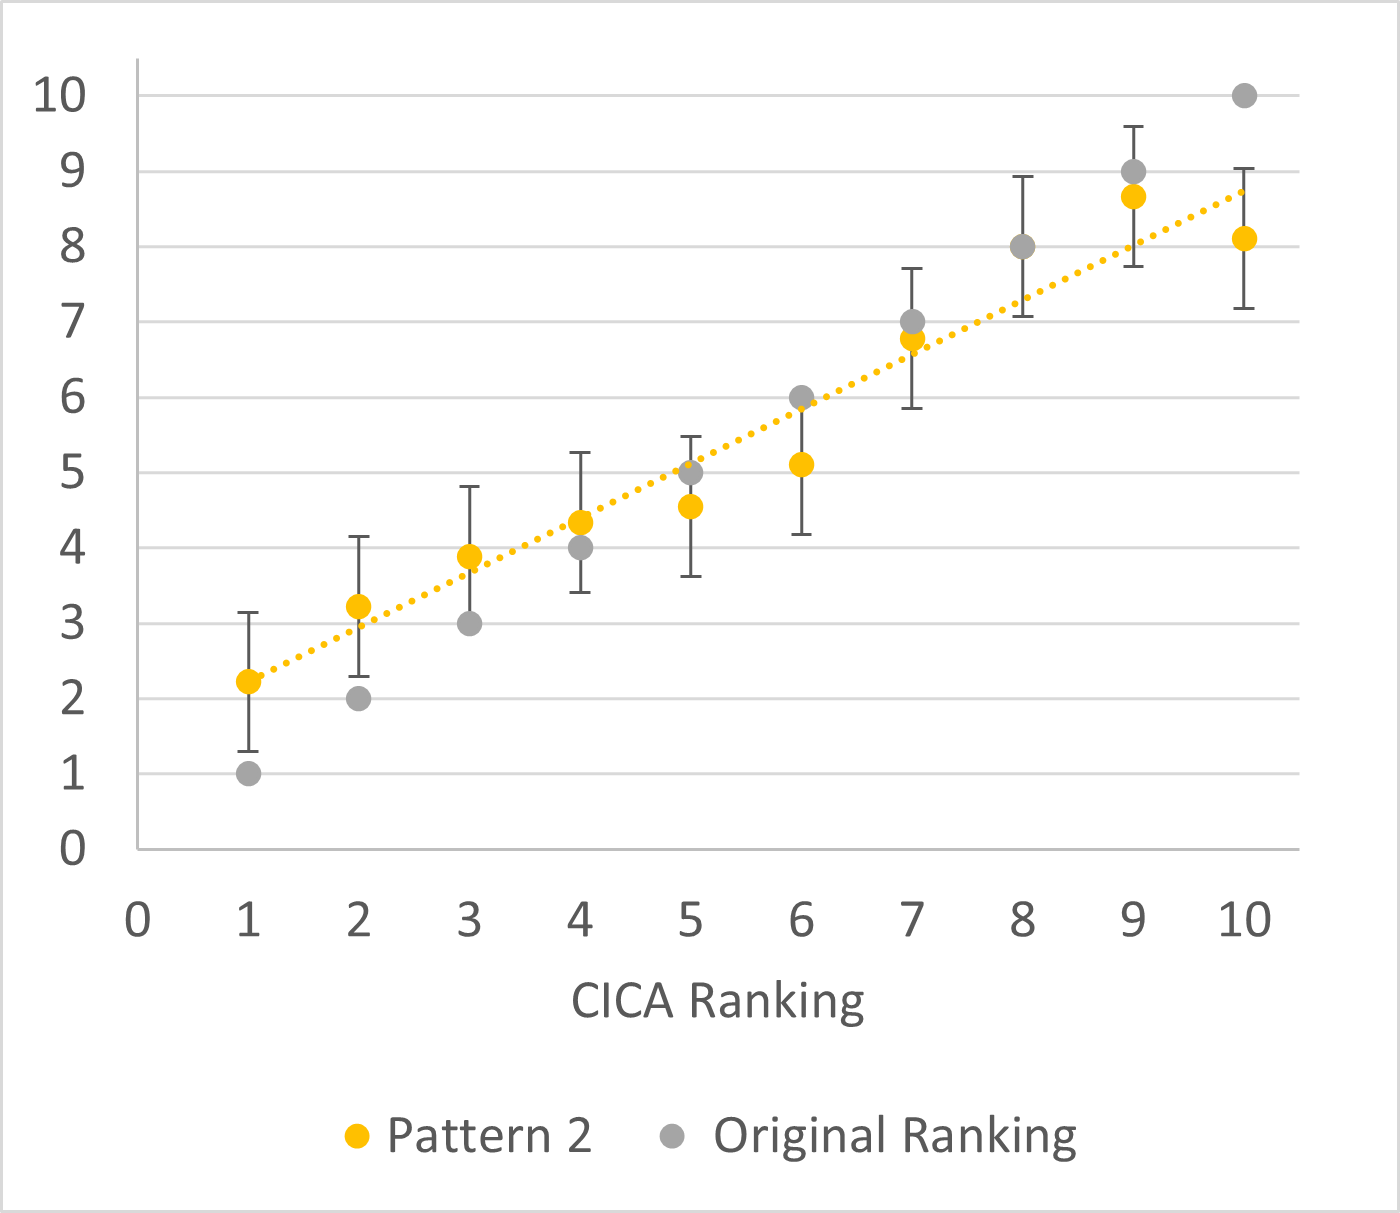
\includegraphics[width=\linewidth]{Images/AccuracyPattern2}
            \captionof{figure}{Accuracy comparison pattern 2 with original ranking}
            \label{fig:AccuracyPattern2} &
            \centering
            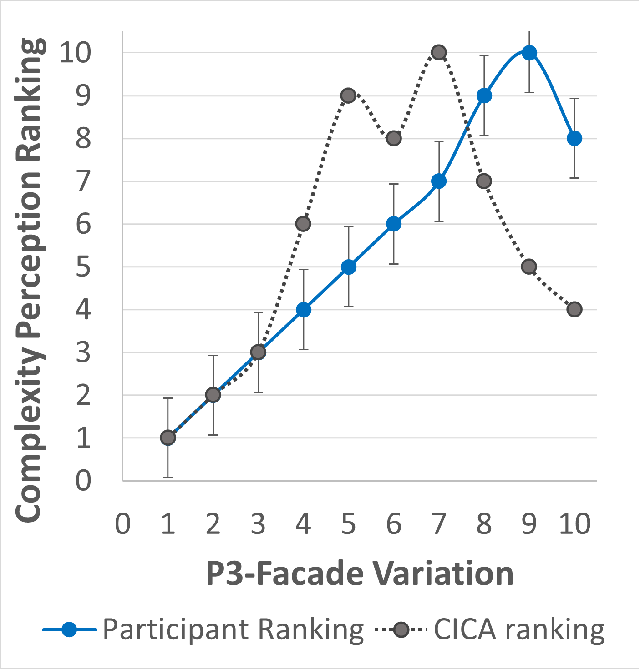
\includegraphics[width=\linewidth]{Images/AccuracyPattern3}
            \captionof{figure}{Accuracy comparison pattern 3 with original ranking}
            \label{fig:AccuracyPattern3}
        \end{tabularx}
    \end{table*}

%!Complexity perception per pattern

The comparison between participant perceptions and the original ranking, as depicted in Figures \ref{fig:AccuracyPattern1}, \ref{fig:AccuracyPattern2}, and \ref{fig:AccuracyPattern3}, highlights how the experiment results closely resemble the shape of the original ranking data, following a similar trajectory.
This analysis aimed to assess the deviation error between the original ranking generated by the CICA system and the ranking established by participants during the 'screen-based ranking' phase of the experiment.

Quantifying this deviation error allowed us to gauge the accuracy of the CICA system in predicting complexity levels in facade design.

The accuracy analysis results, reveal varying degrees of accuracy across facade variations and patterns.
For Pattern 1, in Figure \ref{fig:AccuracyPattern1}, the average deviation is \(SD1 = 0.9\), for Pattern 2, in Figure \ref{fig:AccuracyPattern2}, it is \(SD2 = 0.9\), and for Pattern 3, in Figure \ref{fig:AccuracyPattern3},it is \(SD3 = 1.1\).
Notably, the largest deviation errors tend to occur at both the lowest and highest levels of complexity.


%! Post experiment survey results

The survey results offer valuable insights into how building users perceive facade complexity and the factors influencing their facade design preferences.
The responses to the `complexity perception' section of the survey have been summarized in Figures \ref{fig:SurveyQuestions6-10} and \ref{fig:SurveyQuestions11-15}, with evaluations conducted using a 7-point Likert scale.

  %% Complexity Perception Survey results
    \begin{table*}[htb]
        \centering
        \small
        \begin{tabularx}{\textwidth}{X X}
            \centering
            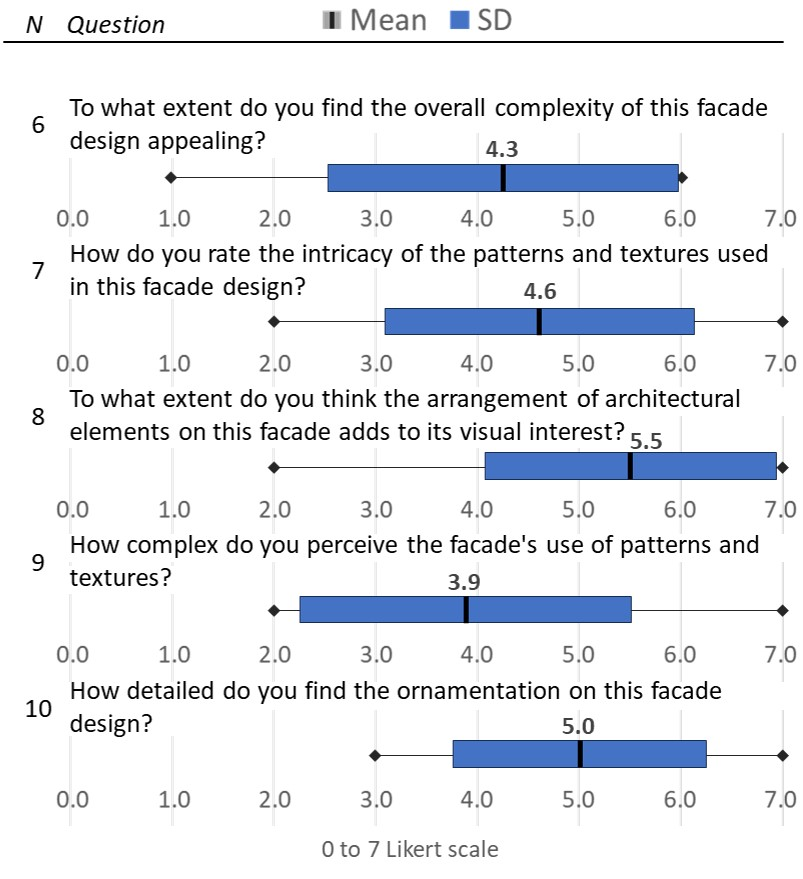
\includegraphics[width=\linewidth]{Images/SurveyPart1Complexity}
            \captionof{figure}{Questions 6 to 10 of the Complexity perception section from the Post-Experiment Survey. \- (n = 10), 1 - strongly disagree, 7 - strongly agree}
            \label{fig:SurveyQuestions6-10} &
            \centering
            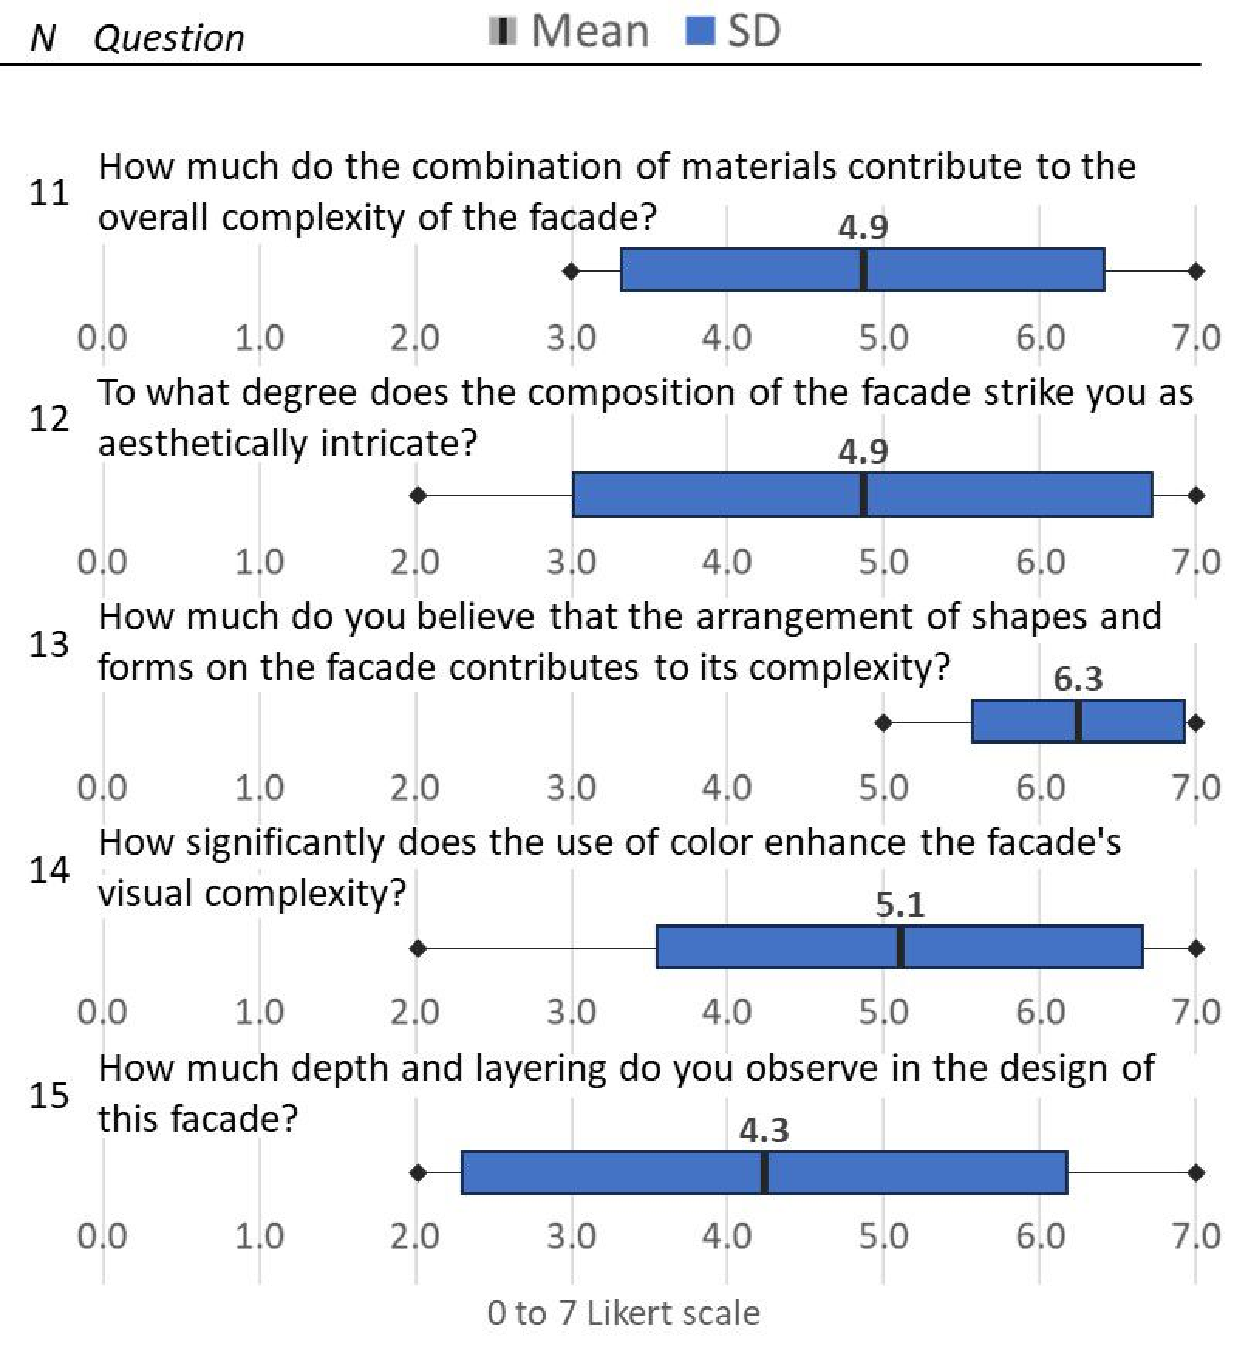
\includegraphics[width=\linewidth]{Images/SurveyPart2Complexity}
            \captionof{figure}{Questions 6 to 10 of the Complexity perception section from the Post-Experiment Survey. \- (n = 10), 1 - strongly disagree, 7 - strongly agree}
            \label{fig:SurveyQuestions11-15}
        \end{tabularx}
    \end{table*}

Notably, all the questions garnered scores exceeding \(3.5\), with an average rating of \(4.9\).
This indicates a generally favorable attitude among respondents toward classifying the presented facade variations as complex.
However, the average standard deviation of \(1.5\) reveals a degree of variability in responses.

In other words, the responses are somewhat scattered around the mean (average).
This dispersion suggests that while some participants provided highly positive ratings (above the mean), others offered less enthusiastic assessments (below the mean).
These variations in responses underscore the diverse perspectives and preferences among participants, enriching our understanding of how users perceive facade complexity.


%! Detailed analysis of survey questions
Further analysis suggests .....................

Regarding the aesthetical appeal of the prepared facade variation design the overall consensus

%! Post experiment interview

During post-experiment interviews, participants were asked to express their views on the relative importance of form and materials when evaluating facade.
Remarkably, the responses were unanimous, with participants consistently favoring form over materials as the more significant criterion.
Additionally, participants indicated a clear preference for a weight distribution of \(80\%\) for form and \(20\%\) for materials in their decision-making process when assessing facade complexity.

Regarding intricate facade designs, another consensus among participants was the emphasis on views.
Given the experiment's location, which affords a front view of the entire campus and a side view facing another building, participants expressed a clear preference for an unobstructed facade on the front view.
They suggested that a facade design capable of framing and enhancing the campus view would be preferable over an intricate pattern.

Conversely, for the side of the building facing the neighboring structure, participants favored intricate patterns that offered increased privacy or complexity.
In this context, the view of the neighboring building was considered less important to preserve, and participants believed that a complex facade could enhance both the building's aesthetic appeal and privacy.

%! Preliminary Conclusion

In summary, the findings align with our initial hypothesis, indicating a trend in contemporary architecture towards increasingly complex facade designs.
This shift is evident not only in the quantitative analysis of historical facade complexity trends, as illustrated in Figure \ref{fig:HistoricalComplexityGraph}, but also in the results of our experimental phase.

Participants in the experiment displayed a clear inclination towards complexity, with an average complexity score \(3.82\) on a 0 to 10 scale.
This suggests ample room for the incorporation of complex forms in contemporary building and facade design.
This observation is further reinforced by the overall positive reception of the facade variations in the post-experiment survey, with an average rating of \(4.9\) on a 7-point Likert scale.
Participants consistently characterized the presented facades as both aesthetic and intricate.

Taken together, these findings support the notion that contemporary architecture is embracing complexity in facade design, marking a departure from more simplistic interpretations of architecture associated with the guidelines of modernist movement.

In the forthcoming discussion section, we delve deeper into these implications and explore the potential effects on future construction practices and architectural design principles.

%! Original alternative for accuracy graphs alternative


 %% Figure Complexity perception per level with trendlines
    \begin{figure*}[htb]
      \centering
      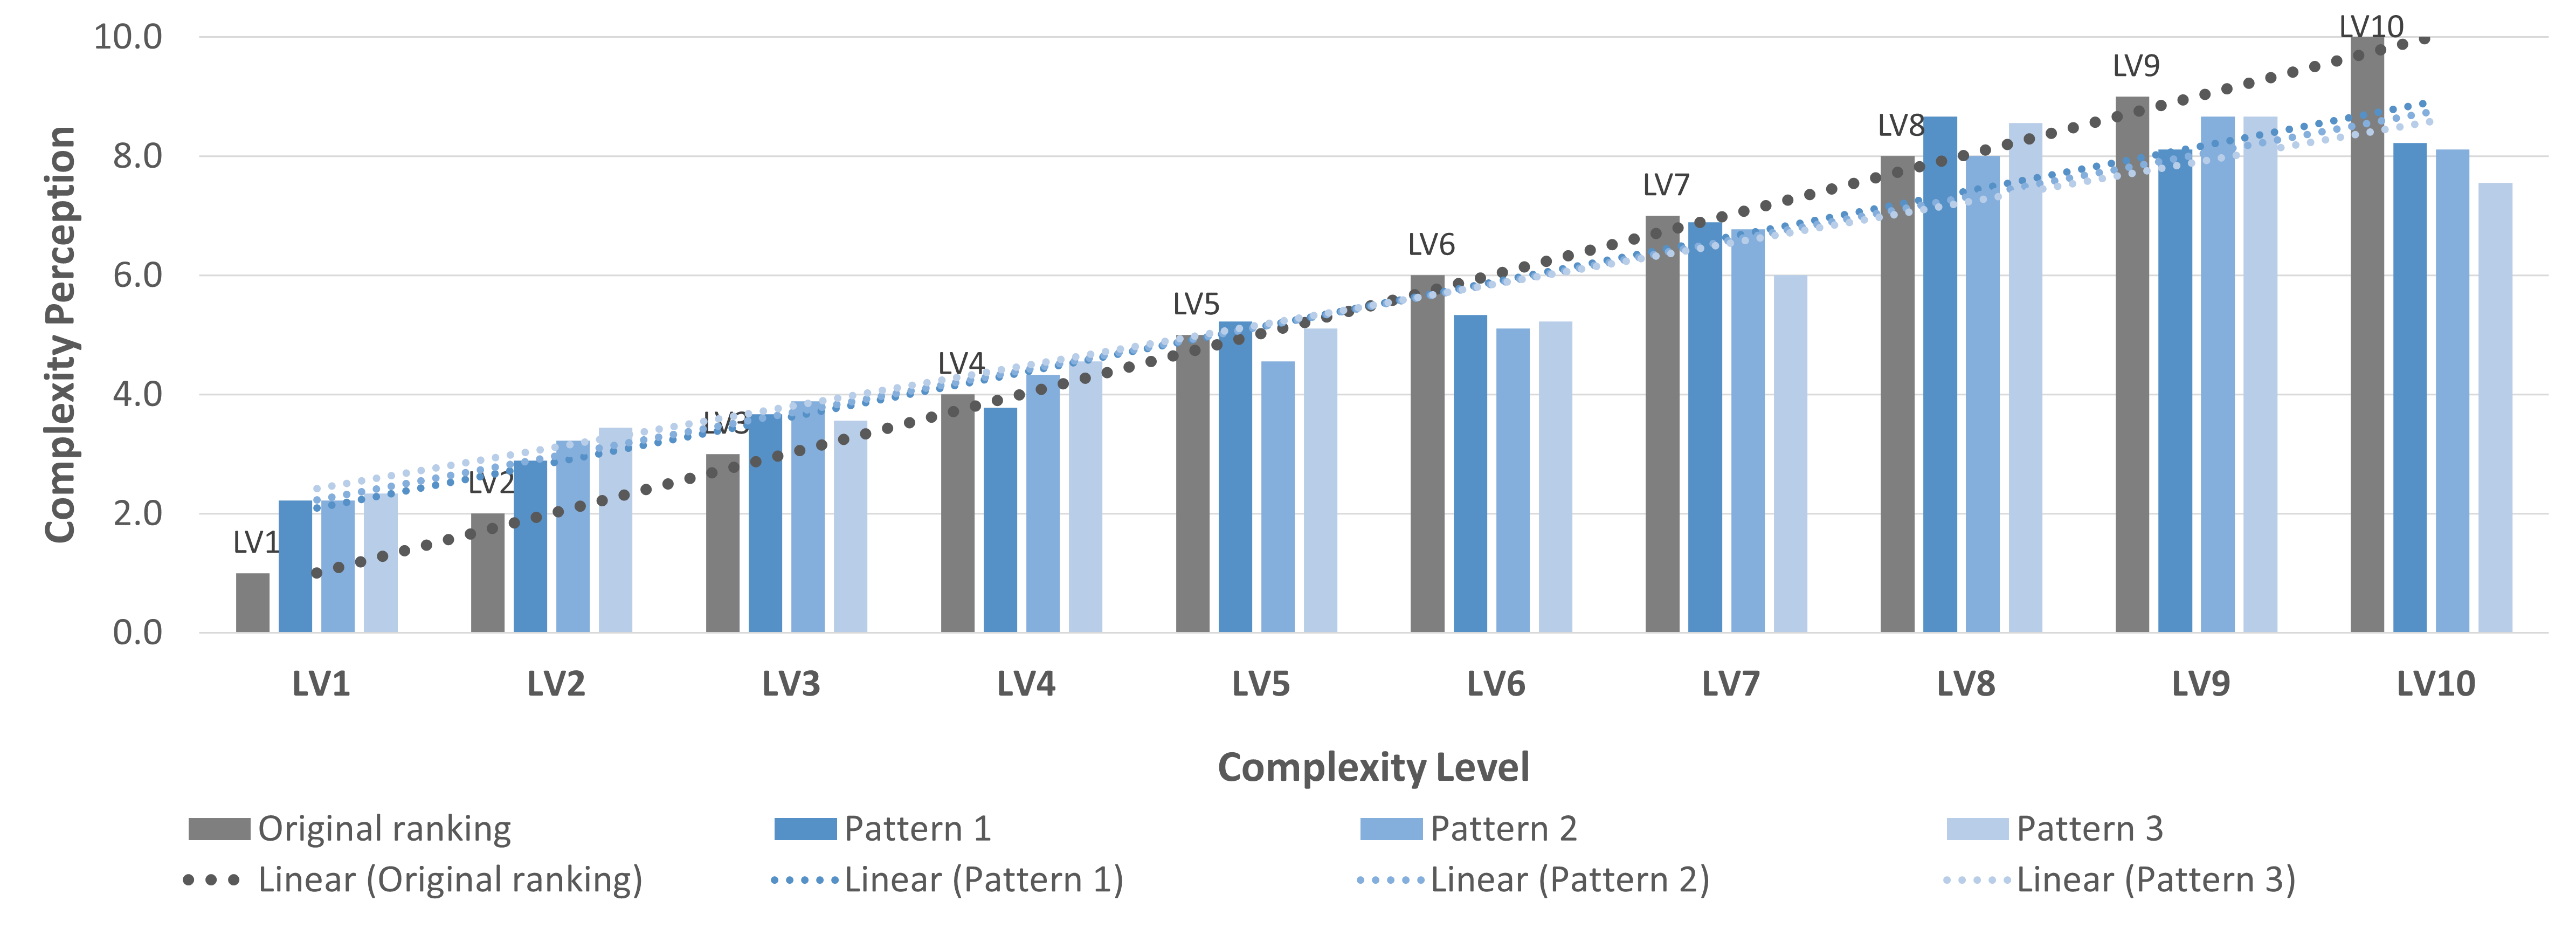
\includegraphics[width= \linewidth, trim=0 0 0 0]{Images/ComplexityPerceptionPerLevel}
      \caption{This graph highlights participants' perception of complexity for the 10 variations within three patterns in contrast to the original ranking. It visually represents the differences between participants' perceived complexity and the initial rankings during the screen-based complexity assessment stage of the experiment.}
      \label{fig:ComplexityPerceptionPerLevel2}
    \end{figure*}

% Old Figure Complexity perception Chart for all patterns
    \begin{figure}[htb]
        \centering
        %trim=100 180 100 120, clip
        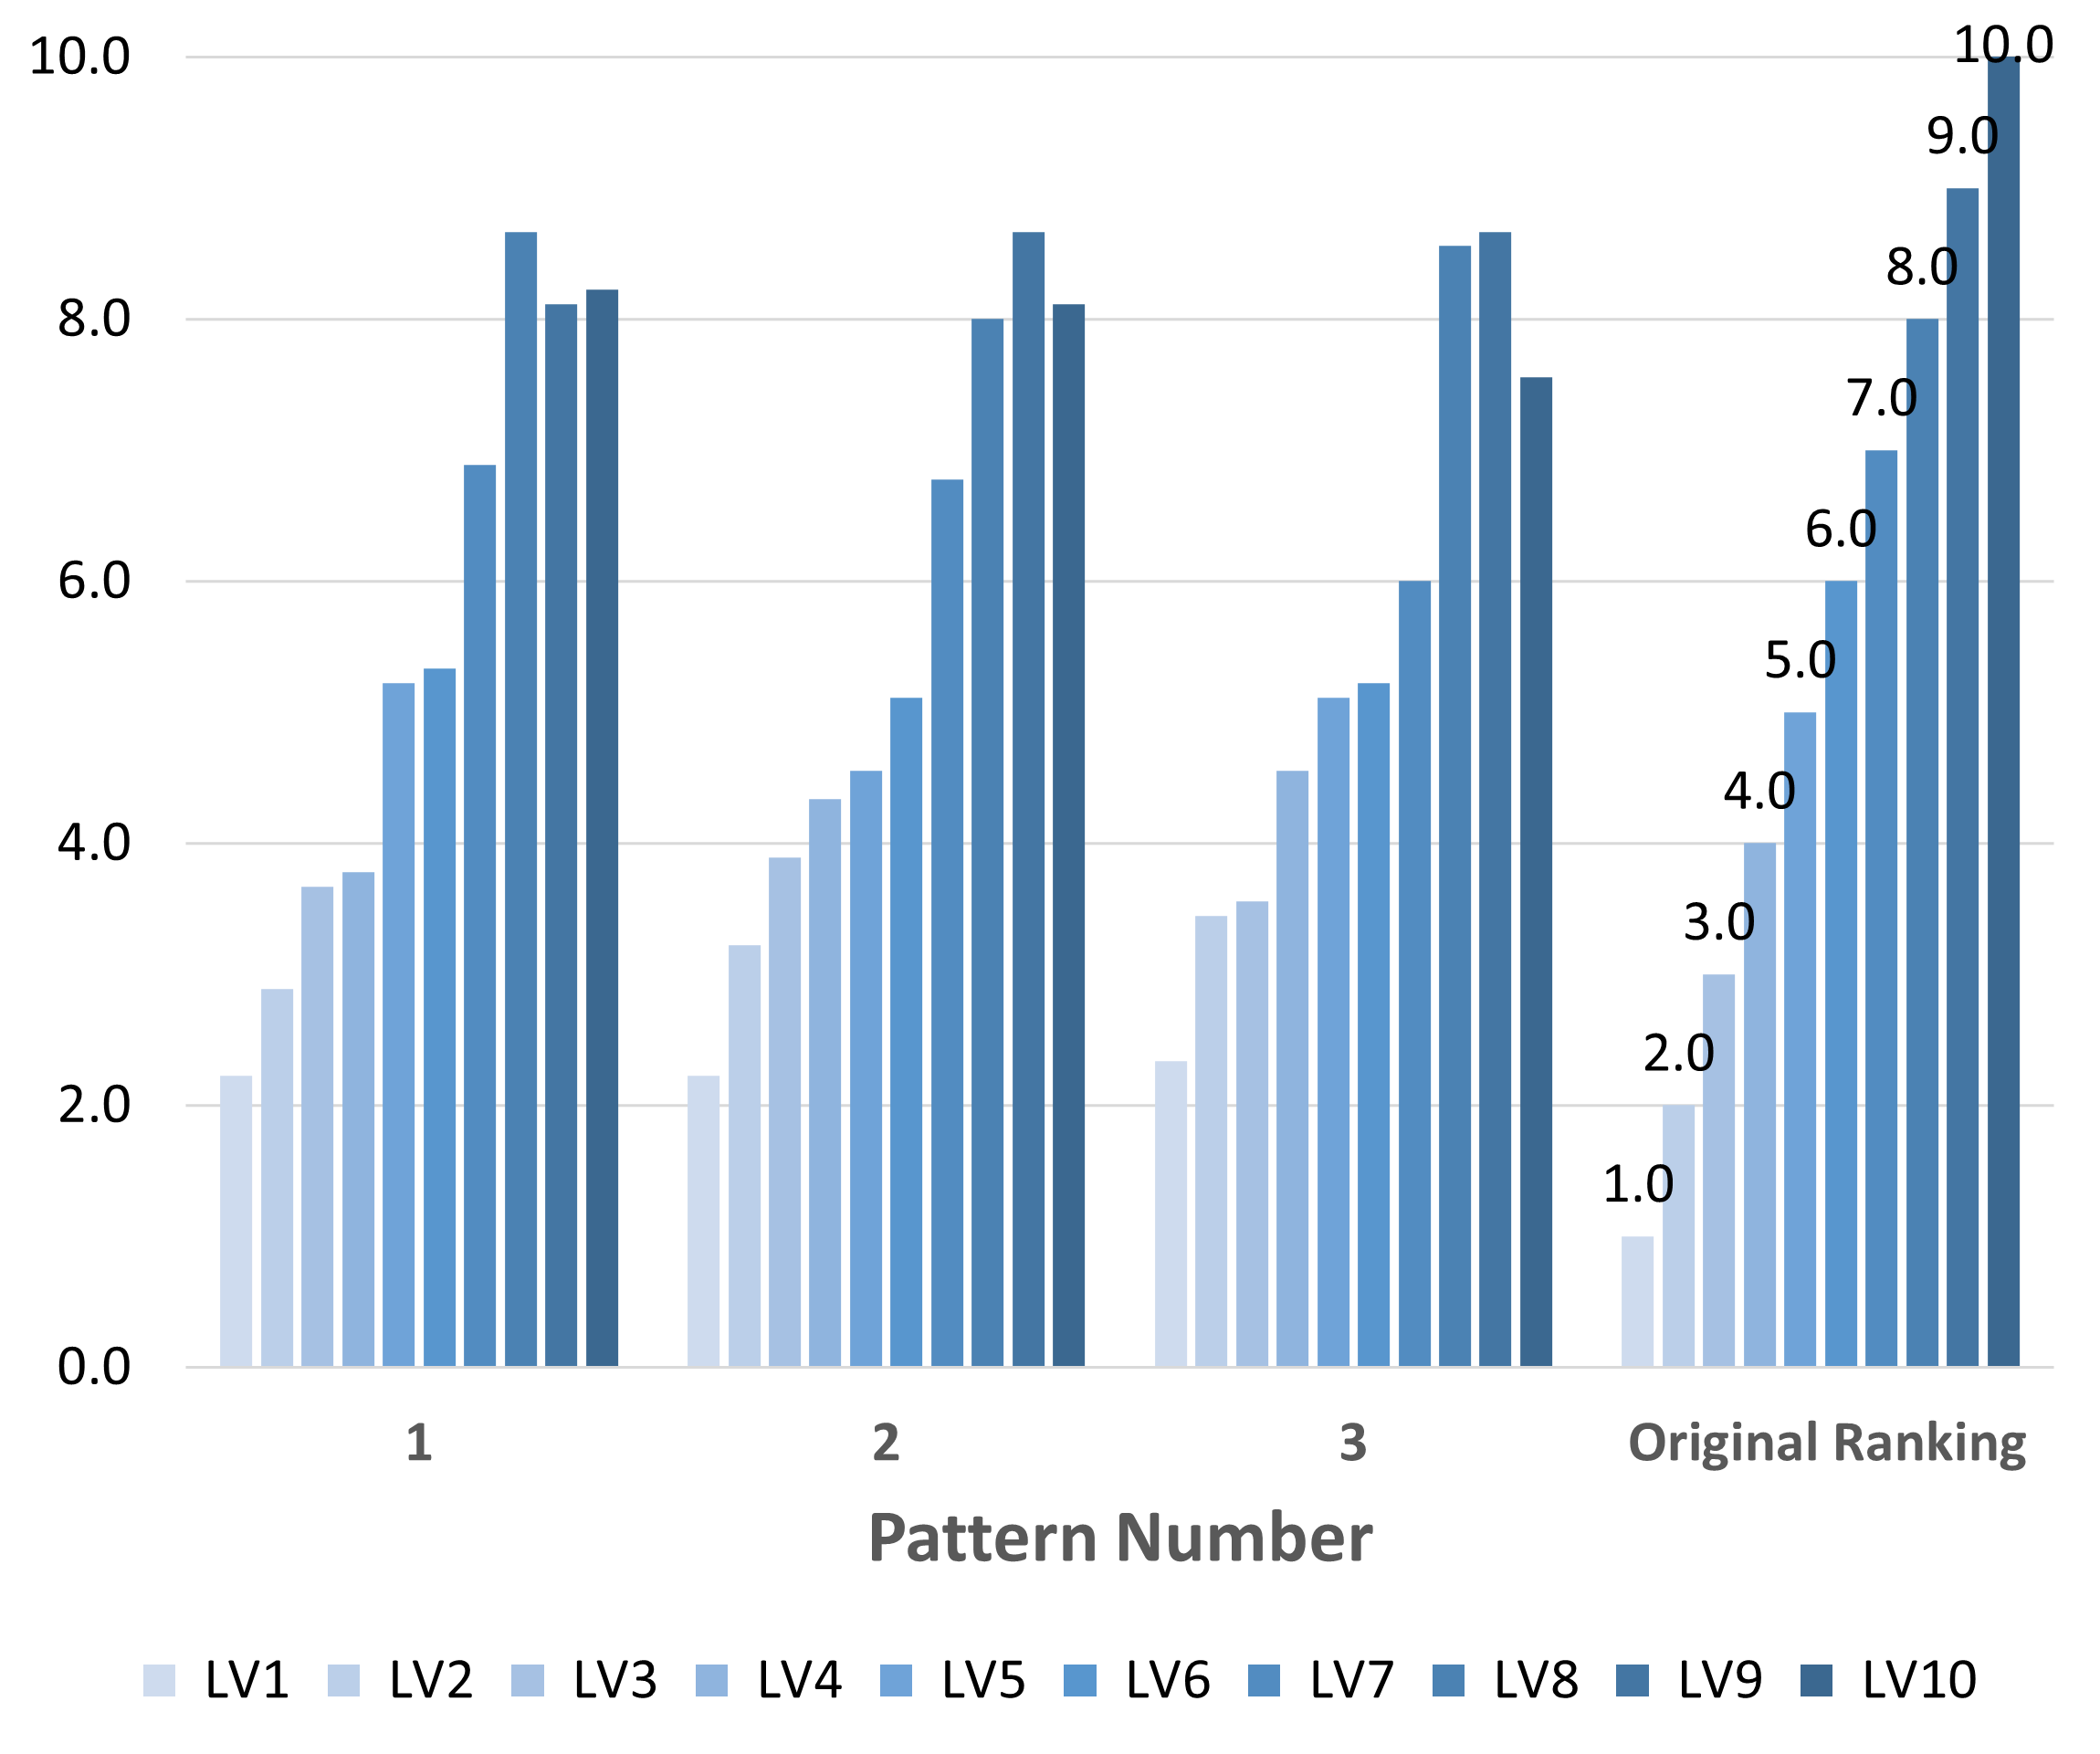
\includegraphics[width=\linewidth]{Images/ComplexityPerceptionChart}
        \caption{Chart depicting participants' complexity perception related to the three patterns. Insights into participants' perception of complexity concerning specific patterns during the screen-based complexity assessment phase of the experiment.}
        \label{fig:ComplexityPerceptionChart}
    \end{figure}

